\documentclass[11pt,a4paper]{report}
\usepackage[utf8]{inputenc}
\usepackage{amsfonts}
\usepackage{pdfpages}
\usepackage{eurosym}
\usepackage{letltxmacro}
\usepackage{microtype}
\usepackage[left=3cm,right=3cm,bottom=3.5cm]{geometry}
\usepackage{fancyhdr}
\usepackage{setspace}
\usepackage{sidecap}
\usepackage{emptypage}
\usepackage{amsmath,amssymb,amsthm, latexsym}
\usepackage{eucal}
\usepackage{eufrak}	
\theoremstyle{definition}
\newtheorem{esercizio}{Esercizio}
\usepackage[english,italian]{babel}
\usepackage{url}
\usepackage{caption}
\captionsetup{tableposition=top,figureposition=bottom,font=small,format=hang,labelfont={sf,bf}}
\usepackage{graphicx}
\usepackage{booktabs}
\usepackage{tabularx}
\usepackage{wrapfig}
\usepackage{subfig}		
\usepackage{siunitx}
\usepackage{makeidx}
\usepackage{mathtools}
\usepackage{pgfplots}
\usepackage{xcolor}
\usepackage{listings}
\usepackage{verbatim}
\usepackage{multirow}
\usepackage{tikz}
\usetikzlibrary{calc}
\usetikzlibrary{positioning}
\usetikzlibrary{matrix}
\usepackage{circuitikz}
\usepackage{hyperref}
\newcommand*\rfrac[2]{{}^{#1}\!/_{#2}}
\usepackage{cancel}
\usepackage{tikz}
\usetikzlibrary{shapes.misc}
\newcommand{\tikzcancel}[2][]{
\tikz[inner sep=0,outer sep=0, remember picture,baseline=(x.base)]\node[anchor=base](x){\ensuremath{#2}};
\tikz[remember picture,overlay,baseline=(x.base)]\draw[-stealth,shorten >=-3pt,shorten <=-3pt,#1] (x.north east)--(x.south west)node{};
}
\usepackage{color}   %May be necessary if you want to color links
\usepackage{hyperref}
\hypersetup{
    colorlinks=true,
    linktoc=page,      
    linkcolor=blue, 
    filecolor = red,
    urlcolor = blue,
    bookmarks=true,
    %pdftoolbar=true,    
}
\usepackage{hyphenat}
\newcommand\AlCentroPagina[1]{%
\AddToShipoutPicture*{\AtPageCenter{%
\makebox(0,0){\includegraphics%
[width =0.9\paperwidth]{#1}}}}}

\begin{document}
\newcommand{\horrule}[1]{\rule{\linewidth}{#1}}
\lstset{language=Java} 
\lstset{basicstyle=\footnotesize\ttfamily}
\author{Silvio Baratto}
\title{
\normalfont \normalsize 
\textsc{Università degli studi di trieste} \\ [25pt] % Your university, school and/or department name(s)
\horrule{0.5pt} \\[0.4cm] % Thin top horizontal rule
\huge Assignment 1\\ % The assignment title
\horrule{2pt} \\[0.5cm] % Thick bottom horizontal rule
}
\maketitle
\tableofcontents
\chapter{section 1}
All the files used for this report are in: \href{https://github.com/SilvioBaratto/HPC}{https://github.com/SilvioBaratto/HPC}
\section{Ring}
%\href{https://github.com/SilvioBaratto}{github}/SilvioBaratto}.\\
This program builds a 1D ring and makes each process sends a message to his right and left neighbour with a tag proportional to its rank. In this way each process add or substracts its rank value depending on which side the message is received. Then each process will resend the messages along the ring until the original message has come back to the original sender. \\
To obtain significant data, I have taken the mean over 10000 repetitions. The figure below shows the time as a function of the number of processors used, as expected the time grows linearly.
\begin{center}
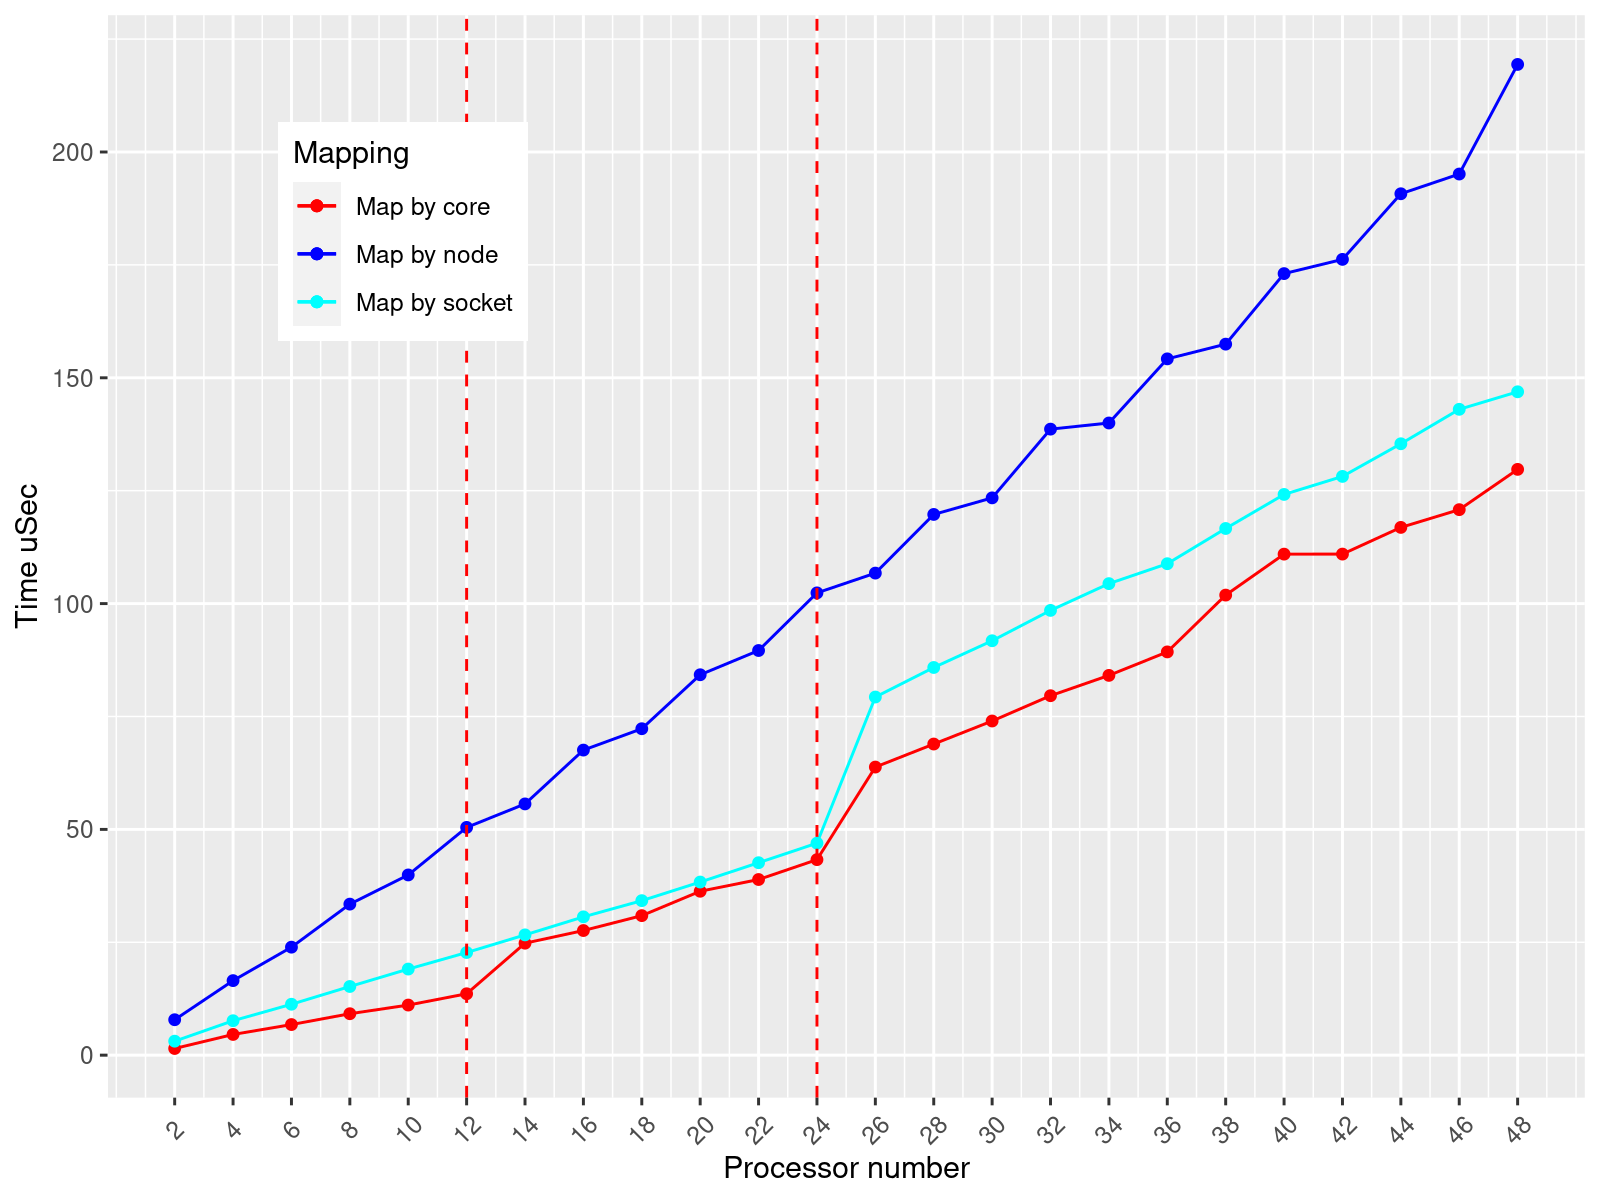
\includegraphics[scale=.45]{ring}
\end{center}
\section{Matrix}
The problem consists in writing a program which performs the sum between 2 3D matrices in parallel, with different virtual topologies.
\subsection{Solution}
A possible solution is to initialize A and B on the root process, then to scatter portions of the 2 matrices to each processes Scatter(), performing the sum between each corresponding block and gathering the results on root Gather().\\
By setting the number of process to 24, three different domains are analyzed for each of the 3 different topologies (1D, 2D and 3D) and the computational time is recorded. The tables do not show any significant differences among the combinations and the topologies.\\
\begin{center}
\begin{tabular}{lll}
\toprule
Distribution & Topology & Time \\
\midrule
(2400 x 100 x 100) & (24, 1, 1) & $0.75044058$ \\
(2400 x 100 x 100) & (12, 2, 1) & $0.69981940$ \\ 
(2400 x 100 x 100) & (6, 2, 2) & $0.75580620$ \\ 
(2400 x 100 x 100) & (4, 3, 2) & $0.70167095$ \\ 
(1200 x 200 x 100) & (24, 1, 1) & $0.74583788$ \\
(1200 x 200 x 100) & (12, 2, 1) & $0.69193223$ \\ 
(1200 x 200 x 100) & (6, 2, 2) & $0.75146050$ \\ 
(1200 x 200 x 100) & (4, 3, 2) & $0.69529179$ \\  
(800 x 300 x 100) & (24, 1, 1) & $0.75275431$ \\
(800 x 300 x 100) & (12, 2, 1) & $0.76012270$ \\  
(800 x 300 x 100) & (6, 2, 2) & $0.69036465$ \\ 
(800 x 300 x 100) & (4, 3, 2) & $0.68957827$ \\ 
\bottomrule
\end{tabular}
\end{center}
\newpage
\chapter{section 2}
\section{MPI PingPong performance}
The PingPong benchmark consists of a message of $N$ bytes sent back and forth between two processes. The output reports the size of the message in number of bytes, the number of repetitions, the communication time in $\mu{s}$ and the effective bandwidth in $Mbytes/s$.\\
The analyses are performed on GPU and Thin nodes. For each type of node, the communication between cores inside the same socket is modeled, across 2 different sockets, and across two different nodes. The assumed model for the communication time is:
\begin{equation*}
T_{comm} = \lambda + \dfrac{m_{size}}{b_{network}}
\end{equation*}
where $\lambda$ is the latency, $m_{size}$ is the size of message, and $b_{network}$ the bandwidth.
%%%% Graphs
\subsubsection{Thin node Openmpi and Intel between sockets and cores}
\textbf{Inside socket}.\\
The plot shows a peak at a message size between $10^{5}$ and $10^{7}$ bytes. To explain this behavior we can consider the caches and the architecture. A single core of a node has an L1-cache of size $32KB$ and L2-cache of $1024KB$. The L2-cache is shared among the cores of one socket. To take measurements the PingPong benchmark, given a small message size repeats the sending of the message several times until it fits in the L1-cache. When the L1-cache is completely full part of the message will be stored inside the L2-cache. The same reasoning can be applied between L2-cache and L3-cache. Up to $1MB$ the message is entirely stored inside the L2-cache, but as the size increases the data retrieved process from L3-cache slows down the process, untill the region inside which the asymptotic bandwidth can be measured is reached.\\
\\
\textbf{Across socket}.\\
Analogous results are obtained when pinning processes across 2 different sockets of the same thin node.\\
\begin{center}
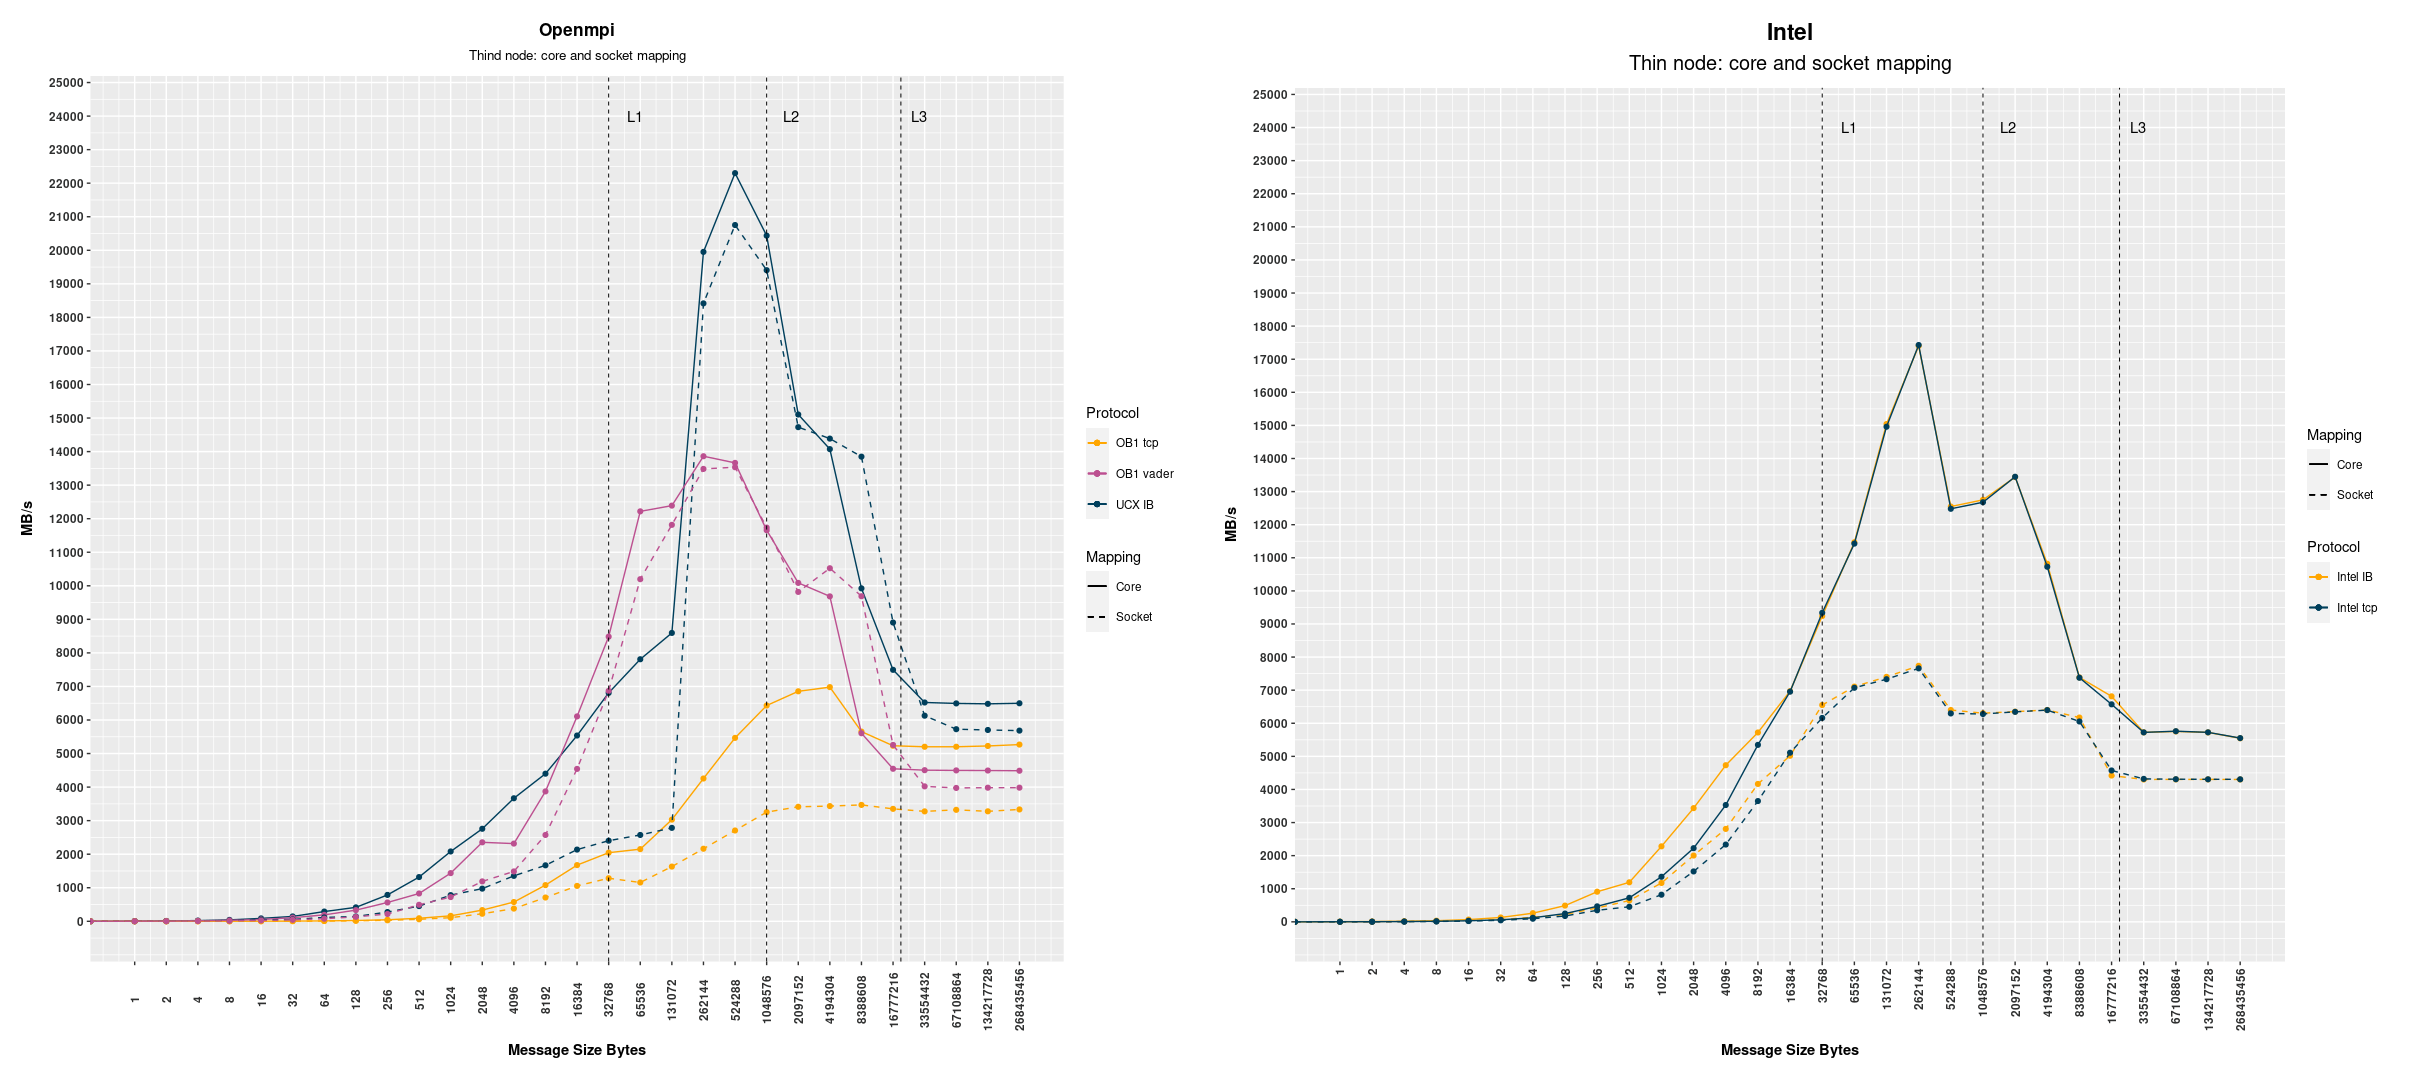
\includegraphics[scale=.25]{thin_intel_openmpi}
\end{center}
\subsubsection{Thin node Openmpi and Intel between sockets and cores}
\begin{center}
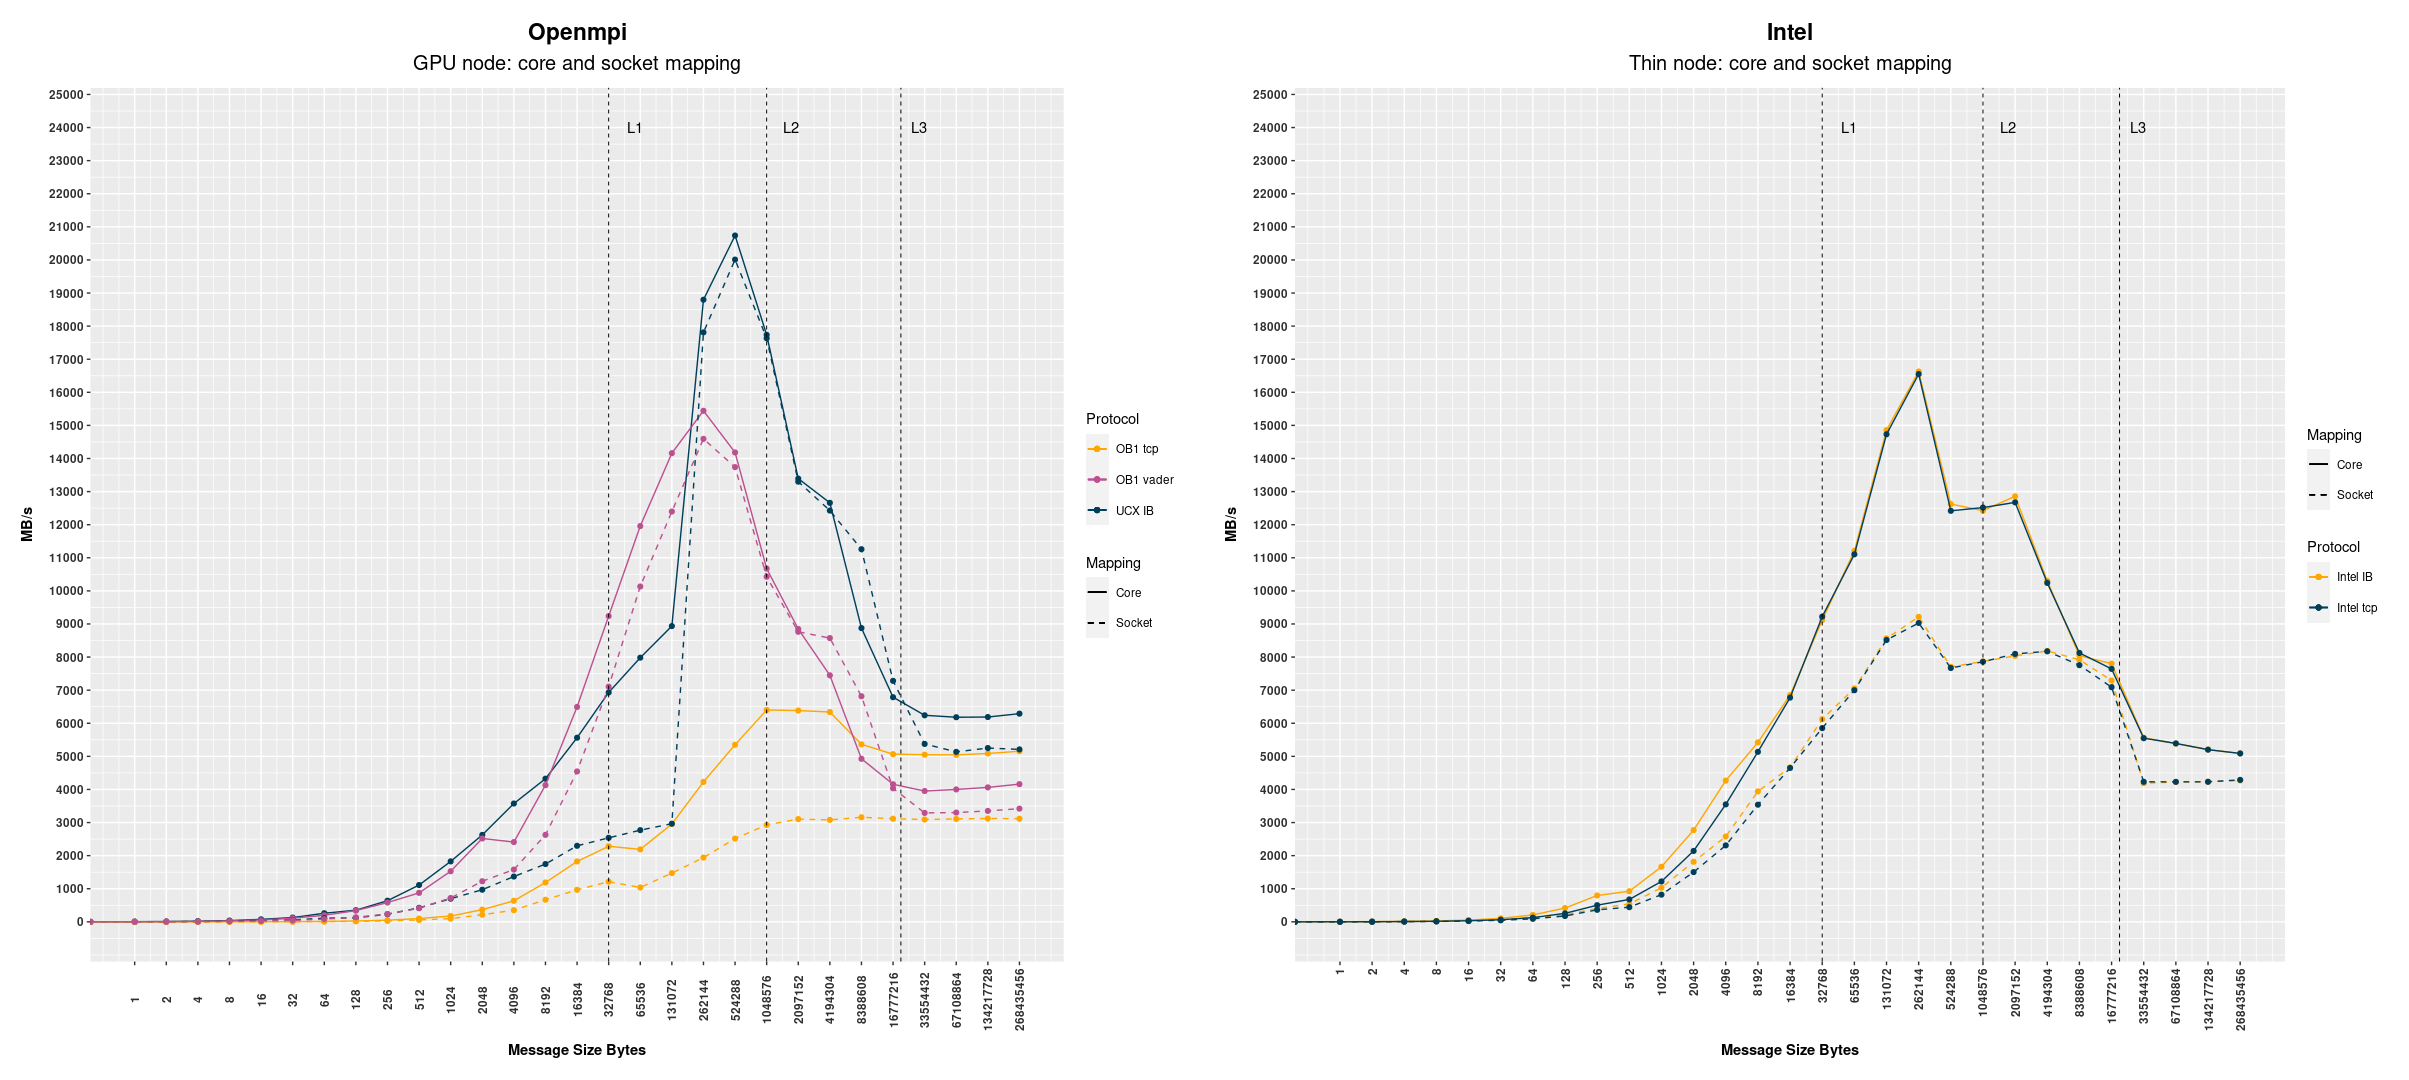
\includegraphics[scale=.25]{gpu_intel_openmpi}
\end{center}
\textbf{Across nodes}.\\
Have observed that without specifying any btl parameter, the messages are exchanged through the 100 Gbit HDR Infiniband which connect the computational nodes in the ORFEO cluster, in this case the values are comparable with the theoretical ones.
\subsubsection{Thin node and Gpu node between nodes}
\begin{center}
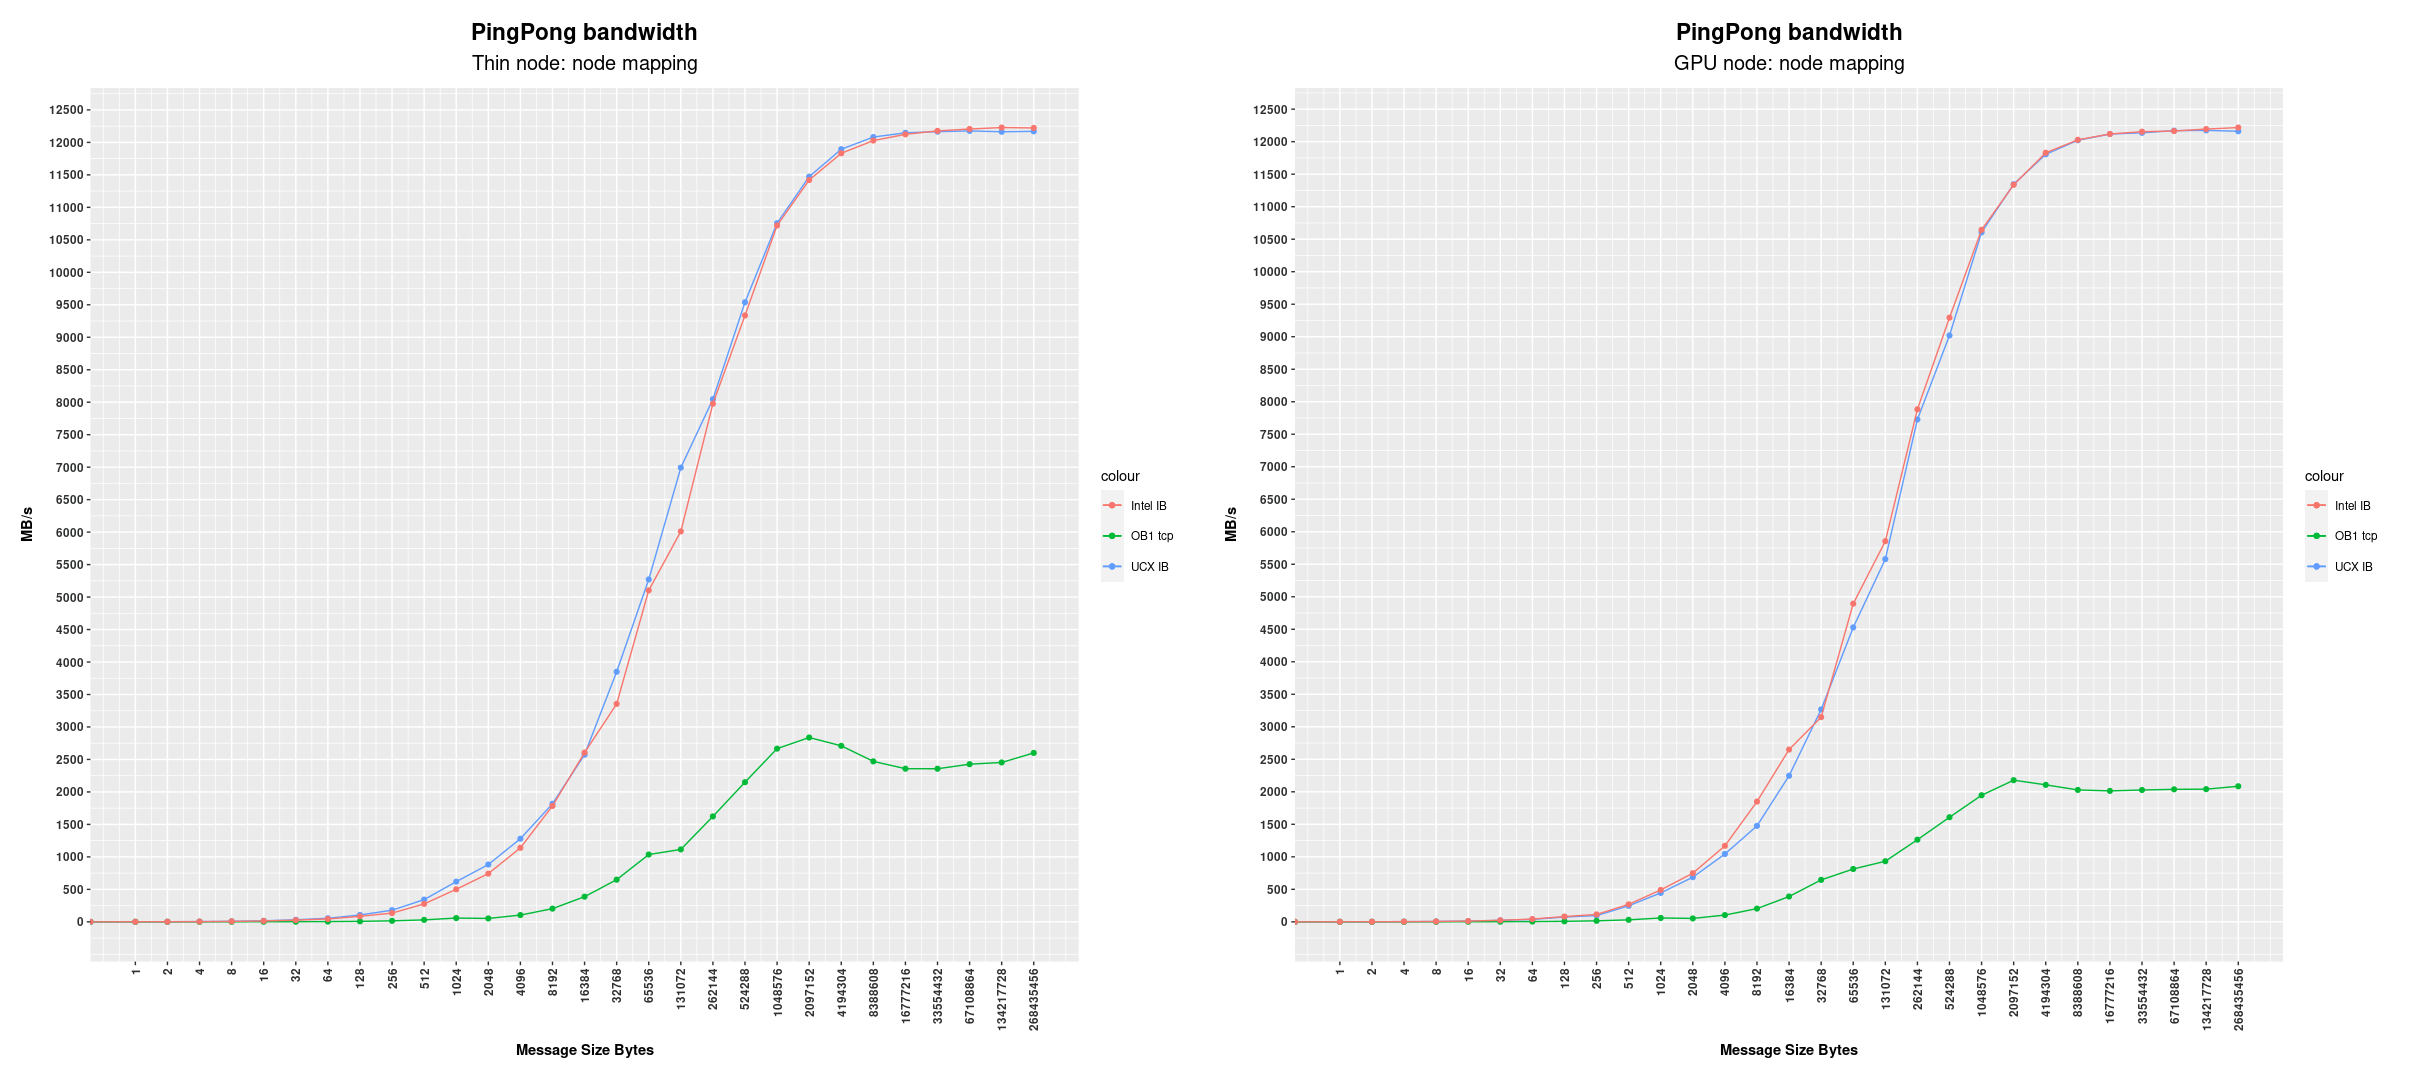
\includegraphics[scale=.25]{node_mapping}
\end{center}
\subsection{Thin node latency and bandwidth}
\begin{center}
\begin{tabular}{clcl}
\toprule
Thin node & Protocol & Latency & Bandwidth  \\
\midrule
\multirow{4}*{Core mapping} & UCX ib  		& $0.22$ 	& $6450.36$ \\
 						     & Intel ib 	& $0.24$ 	& $5702.59$ \\
						     & OB1 vader	& $0.31$ 	& $4472.75$ \\
						     & OB1 tcp		& $5.5$ 	& $5123.82$ \\
\midrule
\multirow{4}*{Socket mapping} 	& UCX ib  		& $0.54$ & $5679.78$ \\
 						     	& Intel ib 		& $0.48$ & $4289.15$ \\
						     	& OB1 vader		& $0.72$ & $3954.68$ \\
						     	& OB1 tcp		& $8.19$ & $3284.49$ \\
\midrule
\multirow{4}*{Node mapping} 	& Openmpi ib  	& $1.07$ 	& $12176.39$ \\
 						     	& Intel ib		& $1.34$ 	& $12235.85$ \\
						     	& OB1 vader		& $1.06$ 	& $12187.99$ \\
						     	& OB1 tcp		& $15.76$ 	& $2402.39$ \\
\bottomrule
\end{tabular}
\end{center}
\subsection{Gpu node latency and bandwidth}
\begin{center}
\begin{tabular}{clcl}
\toprule
Gpu node & Protocol & Latency & Bandwidth  \\
\midrule
\multirow{4}*{Core mapping} & UCX ib  		& $0.26$ 	& $6157.24$ \\
 						     & Intel ib 	& $0.32$ 	& $5216.97$ \\
						     & OB1 vader	& $0.30$ 	& $4030.76$ \\
						     & OB1 tcp		& $5.03$ 	& $5072.48$ \\
\midrule
\multirow{4}*{Socket mapping} 	& UCX ib  		& $0.60$ & $5201.56$ \\
 						     	& Intel ib 		& $0.53$ & $4209.24$ \\
						     	& OB1 vader		& $0.71$ & $3318.39$ \\
						     	& OB1 tcp		& $8.73$ & $3121.66$ \\
\bottomrule
\end{tabular}
\end{center}
\newpage
\chapter{section 3}
\section{Jacobi solver}
\subsection{Performance}
To predict the performance of the Jacobi model we use the following formula:
\begin{equation*}
P(L,N) = \dfrac{L^{3}N}{T_{s} + T_{c}}[MLUP/s]
\end{equation*}
$L$ is the size of cubic sub-domains, $T_{s}$ is the time for the lattice updates of a domain with size $L$ and $T_{c}$ is the communication time.  The quantity $T_{s}$ can be modeled estimating the latency $\lambda$, bandwidth $B$ and messages size $C$.  
\begin{equation*}
T_{c} = \dfrac{C(L,N)}{B} + 4k\lambda [s]
\end{equation*}
$C(L,N)$ is the maximum bidirectional bandwidth data volume transferred over a node's network link, $k$ is the largest number of coordinate directions in which the number of processes is greater than one and $\lambda$ is the latency. The formula for $C$ is:
\begin{equation*}
C = L^{2} \times k \times 2 \times 8 [byte]
\end{equation*}
\subsection{Results}
The following tables compare the results obtained by running Jacobi with the performance model. In thin nodes, the performance $P(N,L)$ predicted from theoretical models reflect the real performance obtained from computation well. In Gpu nodes, instead there is an overestimation from the model, this could happen because hyper-threading enabled is on this node. 
\subsubsection{Thin node, core mapping}
$\lambda = 0.22$, Bandwidth $= 6450.36$
\begin{center}
\begin{tabular}{llllllll} %fatto
\toprule
N & k & C[Mb] & Tc/s & MLUP/s est & MLUP/s real & MLUP/s diff &NP(1)P(N) \\
\midrule
1  & 2	& $46.08$	& $0.00714423$ 	& $112.741 $ 	& $112.738$ 	& $-0.00312003$ & $1$ \\
4  & 4	& $92.16$	& $0.0142885$	& $450.755$		& $451.917$		& $1.16281$ & $0.997864$\\
8  & 6	& $138.24$	& $0.0214327$ 	& $901.089$		& $890.34$		& $-10.749$ & $1.01299$\\
12 & 6	& $138.24$	& $0.0214327$	& $1351.63$		& $1325.43$		& $-26.2079$ & $1.0207$\\
\bottomrule
\end{tabular}
\end{center}
\subsubsection{Thin node, socket mapping} %fatto 
$\lambda = 0.54$, Bandwidth $= 5679.78$
\begin{center}
\begin{tabular}{llllllll} 
\toprule
N & k & C[Mb] & Tc/s & MLUP/s est & MLUP/s real & MLUP/s diff &NP(1)P(N) \\
\midrule
1 & 2	& $46.08 $	& $0.00811407$ 	& $112.734$ 	& $112.738$ 	& $0.00401334$ & $1$ \\
4 & 4	& $92.16$	& $0.0162281$	& $450.698$		& $447.417$		& $-3.28006$ & $1.0079$\\
8 & 6	& $138.24$	& $0.0243422$ 	& $900.918$		& $883.429$		& $-17.4894$ & $1.02091$\\
12& 6	& $138.24$	& $0.0243422$	& $1351.38$		& $1336.19$		& $-15.1886$ & $2.09478$\\
\bottomrule
\end{tabular}
\end{center}
\subsubsection{Thin node, node mapping} %fatto
$\lambda = 1.07$, Bandwidth $= 12176.39$
\begin{center}
\begin{tabular}{llllllll}
\toprule
N & k & C[Mb] & Tc/s & MLUP/s est & MLUP/s real & MLUP/s diff &NP(1)P(N) \\
\midrule
1 & 2	& $46.08$	& $0.00378651$ 	& $112.766$	 	& $112.738$ 	& $-0.0278236$ & $1$ \\
12& 6	& $138.24$	& $0.0113595$	& $1352.52$		& $1326.58$		& $-25.942$ & $1.01981$\\
24& 6	& $138.24$	& $0.0113595$ 	& $2705.04$		& $2627.13$		& $-77.913$ & $1.02991$\\
48& 6	& $138.24$	& $0.0113595$	& $5410.09$		& $5131.27$		& $-278.814$ & $1.0546$\\
\bottomrule
\end{tabular}
\end{center}
\subsubsection{Gpu node, core mapping} 
$\lambda = 0.26$, Bandwidth $= 6157.24$
\begin{center}
\begin{tabular}{llllllll} %fatto
\toprule
N & k & C[Mb] & Tc/s & MLUP/s est & MLUP/s real & MLUP/s diff &NP(1)P(N) \\
\midrule
1 &2	& $46.08$	& $0.00748439$ 	& $78.1282$ 	& $78.1421$ 	& $0.0138761$ & $1$ \\
4&4		& $92.16$	& $0.0149688$	& $312.407$		& $309.684$		& $-2.72303$ & $1.00931$\\
8&6		& $138.24$	& $0.0224532$ 	& $624.603$		& $586.338$		& $-38.2651$ & $1.06617$\\
12&6	& $138.24$	& $0.0224532$	& $936.905$		& $850.567$		& $-86.3376$ & $1.10245$\\
\bottomrule
\end{tabular}
\end{center}
\subsubsection{Gpu node, socket mapping}
$\lambda = 0.60$, Bandwidth $= 5201.56$
\begin{center}
\begin{tabular}{llllllll} %fatto
\toprule
N & k & C[Mb] & Tc/s & MLUP/s est & MLUP/s real & MLUP/s diff &NP(1)P(N) \\
\midrule
1 &2	& $46.08$	& $0.00886008$ 	& $78.1234$ 	& $78.1421$ 	& $0.0187353$ & $1$ \\
4 &4	    & $92.16$	& $0.0177202$	& $312.368$		& $311.43$		& $-0.938776$ & $1.00366$\\
8 &6	& $138.24$	& $0.0265802$ 	& $624.487$		& $611.262$		& $-13.2245$ & $1.0227$\\
12&6	& $138.24$	& $0.0265802$	& $936.73$		& $899.664$		& $-37.066$ & $1.04228$\\
\bottomrule
\end{tabular}
\end{center}
\subsubsection{Gpu node, node mapping} %fatto
$\lambda = 1.58$, Bandwidth $= 12185.46$
\begin{center}
\begin{tabular}{llllllll}
\toprule
N & k & C[Mb] & Tc/s & MLUP/s est & MLUP/s real & MLUP/s diff &NP(1)P(N) \\
\midrule
1 &2	& $46.08$	& $0.00378472$ 	& $78.1413$ 	& $78.1421$ 	& $0.000805104$ & $1$ \\
12&6	& $138.24$	& $0.0113541$	& $937.375$		& $897.053$		& $-40.3223$ & $1.04532$\\
24&6	& $138.24$	& $0.0113541$ 	& $1874.75$		& $1686.53$		& $-188.224$ & $1.112$\\
48&6	& $138.24$	& $0.0113541$	& $3749.5$		& $2488.66$		& $-1260.83$ & $1.50716$\\
\bottomrule
\end{tabular}
\end{center}
The biggest difference between model and data is the communication time. In fact, the time $T_c$ predicted from the model is hundred time smaller then the observed one. However, the simple model used is good enough to predict the performance of the program.
\end{document}
